\documentclass{standalone}
\usepackage{tikz}
\usetikzlibrary{patterns, positioning}

\begin{document}
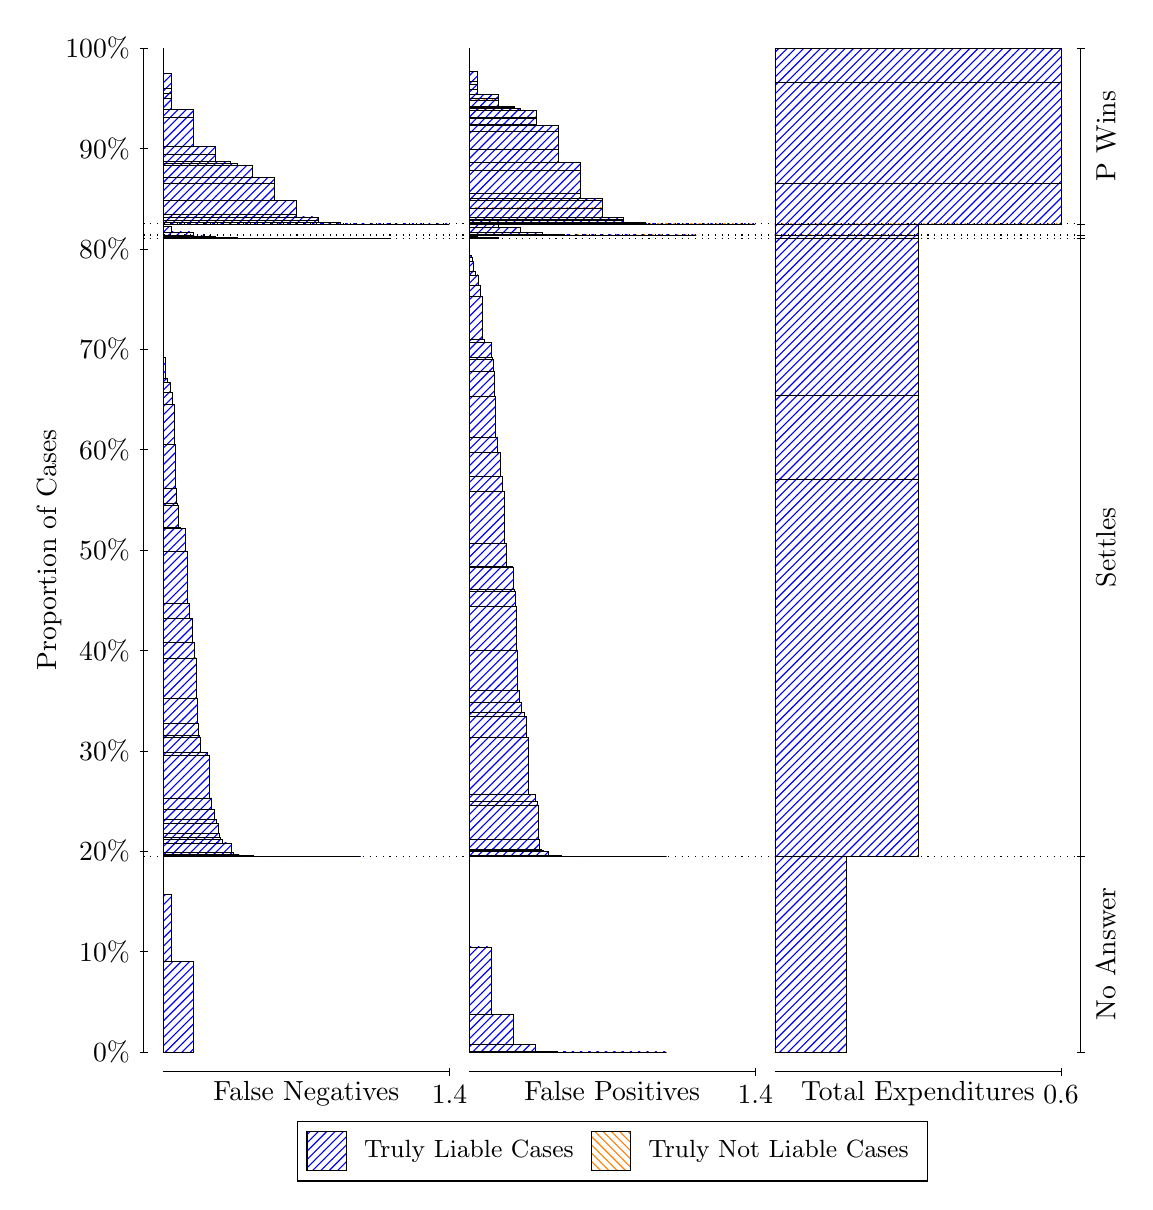
\begin{tikzpicture}
\draw[black, very thin] (1.5,1.75) -- (1.5,14.5);
\node[rotate=90, anchor=center] at (0.3, 8.125) {Proportion of Cases};
\draw[black, very thin] (1.45,1.75) -- (1.55,1.75);
\node[anchor=east] at (1.45, 1.75) {0\%};
\draw[black, very thin] (1.45,3.025) -- (1.55,3.025);
\node[anchor=east] at (1.45, 3.025) {10\%};
\draw[black, very thin] (1.45,4.3) -- (1.55,4.3);
\node[anchor=east] at (1.45, 4.3) {20\%};
\draw[black, very thin] (1.45,5.575) -- (1.55,5.575);
\node[anchor=east] at (1.45, 5.575) {30\%};
\draw[black, very thin] (1.45,6.85) -- (1.55,6.85);
\node[anchor=east] at (1.45, 6.85) {40\%};
\draw[black, very thin] (1.45,8.125) -- (1.55,8.125);
\node[anchor=east] at (1.45, 8.125) {50\%};
\draw[black, very thin] (1.45,9.4) -- (1.55,9.4);
\node[anchor=east] at (1.45, 9.4) {60\%};
\draw[black, very thin] (1.45,10.675) -- (1.55,10.675);
\node[anchor=east] at (1.45, 10.675) {70\%};
\draw[black, very thin] (1.45,11.95) -- (1.55,11.95);
\node[anchor=east] at (1.45, 11.95) {80\%};
\draw[black, very thin] (1.45,13.225) -- (1.55,13.225);
\node[anchor=east] at (1.45, 13.225) {90\%};
\draw[black, very thin] (1.45,14.5) -- (1.55,14.5);
\node[anchor=east] at (1.45, 14.5) {100\%};

\draw[black, very thin] (13.4,1.75) -- (13.4,14.5);
\draw[black, very thin] (13.35,1.75) -- (13.45,1.75);
\node[anchor=west] at (13.35, 1.75) {};
\draw[black, very thin] (13.35,4.2363) -- (13.45,4.2363);
\node[anchor=west] at (13.35, 4.2363) {};
\draw[black, very thin] (13.35,12.083) -- (13.45,12.083);
\node[anchor=west] at (13.35, 12.083) {};
\draw[black, very thin] (13.35,12.126) -- (13.45,12.126);
\node[anchor=west] at (13.35, 12.126) {};
\draw[black, very thin] (13.35,12.267) -- (13.45,12.267);
\node[anchor=west] at (13.35, 12.267) {};
\draw[black, very thin] (13.35,14.5) -- (13.45,14.5);
\node[anchor=west] at (13.35, 14.5) {};

\draw[black, very thin, pattern color=blue, pattern=north east lines] (1.75,1.75) rectangle (2.1259,2.9018);
\draw[black, very thin, pattern color=blue, pattern=north east lines] (1.75,2.9018) rectangle (1.8474,3.7553);
\draw[black, very thin, pattern color=orange, pattern=north west lines] (1.75,3.7553) rectangle (1.75,3.7553);
\draw[black, very thin, pattern color=blue, pattern=north east lines] (1.75,3.7553) rectangle (1.75,4.2363);
\draw[black, very thin, pattern color=blue, pattern=north east lines] (1.75,4.2363) rectangle (4.2557,4.2363);
\draw[black, very thin, pattern color=blue, pattern=north east lines] (1.75,4.2363) rectangle (4.1305,4.2363);
\draw[black, very thin, pattern color=blue, pattern=north east lines] (1.75,4.2363) rectangle (4.0052,4.2363);
\draw[black, very thin, pattern color=blue, pattern=north east lines] (1.75,4.2363) rectangle (3.9773,4.2363);
\draw[black, very thin, pattern color=blue, pattern=north east lines] (1.75,4.2363) rectangle (3.8799,4.2363);
\draw[black, very thin, pattern color=blue, pattern=north east lines] (1.75,4.2363) rectangle (3.852,4.2363);
\draw[black, very thin, pattern color=blue, pattern=north east lines] (1.75,4.2363) rectangle (3.7546,4.2363);
\draw[black, very thin, pattern color=blue, pattern=north east lines] (1.75,4.2363) rectangle (3.7268,4.2363);
\draw[black, very thin, pattern color=blue, pattern=north east lines] (1.75,4.2363) rectangle (3.6989,4.2363);
\draw[black, very thin, pattern color=blue, pattern=north east lines] (1.75,4.2363) rectangle (3.6293,4.2363);
\draw[black, very thin, pattern color=blue, pattern=north east lines] (1.75,4.2363) rectangle (3.6015,4.2363);
\draw[black, very thin, pattern color=blue, pattern=north east lines] (1.75,4.2363) rectangle (3.5736,4.2363);
\draw[black, very thin, pattern color=blue, pattern=north east lines] (1.75,4.2363) rectangle (3.504,4.2363);
\draw[black, very thin, pattern color=blue, pattern=north east lines] (1.75,4.2363) rectangle (3.4762,4.2363);
\draw[black, very thin, pattern color=blue, pattern=north east lines] (1.75,4.2363) rectangle (3.4483,4.2363);
\draw[black, very thin, pattern color=blue, pattern=north east lines] (1.75,4.2363) rectangle (3.4205,4.2363);
\draw[black, very thin, pattern color=blue, pattern=north east lines] (1.75,4.2363) rectangle (3.3787,4.2363);
\draw[black, very thin, pattern color=blue, pattern=north east lines] (1.75,4.2363) rectangle (3.3509,4.2363);
\draw[black, very thin, pattern color=blue, pattern=north east lines] (1.75,4.2363) rectangle (3.3231,4.2363);
\draw[black, very thin, pattern color=blue, pattern=north east lines] (1.75,4.2363) rectangle (3.2952,4.2363);
\draw[black, very thin, pattern color=blue, pattern=north east lines] (1.75,4.2363) rectangle (3.2534,4.2363);
\draw[black, very thin, pattern color=blue, pattern=north east lines] (1.75,4.2363) rectangle (3.2256,4.2363);
\draw[black, very thin, pattern color=blue, pattern=north east lines] (1.75,4.2363) rectangle (3.1978,4.2363);
\draw[black, very thin, pattern color=blue, pattern=north east lines] (1.75,4.2363) rectangle (3.1699,4.2364);
\draw[black, very thin, pattern color=blue, pattern=north east lines] (1.75,4.2364) rectangle (3.1421,4.2364);
\draw[black, very thin, pattern color=blue, pattern=north east lines] (1.75,4.2364) rectangle (3.1003,4.2364);
\draw[black, very thin, pattern color=blue, pattern=north east lines] (1.75,4.2364) rectangle (3.0725,4.2364);
\draw[black, very thin, pattern color=blue, pattern=north east lines] (1.75,4.2364) rectangle (3.0446,4.2364);
\draw[black, very thin, pattern color=blue, pattern=north east lines] (1.75,4.2364) rectangle (3.0168,4.2364);
\draw[black, very thin, pattern color=blue, pattern=north east lines] (1.75,4.2364) rectangle (3.0029,4.2365);
\draw[black, very thin, pattern color=blue, pattern=north east lines] (1.75,4.2365) rectangle (2.975,4.2365);
\draw[black, very thin, pattern color=blue, pattern=north east lines] (1.75,4.2365) rectangle (2.9472,4.2366);
\draw[black, very thin, pattern color=blue, pattern=north east lines] (1.75,4.2366) rectangle (2.9193,4.2371);
\draw[black, very thin, pattern color=blue, pattern=north east lines] (1.75,4.2371) rectangle (2.8915,4.2428);
\draw[black, very thin, pattern color=blue, pattern=north east lines] (1.75,4.2428) rectangle (2.8637,4.2428);
\draw[black, very thin, pattern color=blue, pattern=north east lines] (1.75,4.2428) rectangle (2.8219,4.2428);
\draw[black, very thin, pattern color=blue, pattern=north east lines] (1.75,4.2428) rectangle (2.7941,4.2428);
\draw[black, very thin, pattern color=blue, pattern=north east lines] (1.75,4.2428) rectangle (2.7662,4.2429);
\draw[black, very thin, pattern color=blue, pattern=north east lines] (1.75,4.2429) rectangle (2.7523,4.2439);
\draw[black, very thin, pattern color=blue, pattern=north east lines] (1.75,4.2439) rectangle (2.7384,4.2463);
\draw[black, very thin, pattern color=blue, pattern=north east lines] (1.75,4.2463) rectangle (2.7245,4.2529);
\draw[black, very thin, pattern color=blue, pattern=north east lines] (1.75,4.2529) rectangle (2.6966,4.2553);
\draw[black, very thin, pattern color=blue, pattern=north east lines] (1.75,4.2553) rectangle (2.6688,4.265);
\draw[black, very thin, pattern color=blue, pattern=north east lines] (1.75,4.265) rectangle (2.6409,4.2855);
\draw[black, very thin, pattern color=blue, pattern=north east lines] (1.75,4.2855) rectangle (2.6131,4.4038);
\draw[black, very thin, pattern color=blue, pattern=north east lines] (1.75,4.4038) rectangle (2.5852,4.4054);
\draw[black, very thin, pattern color=blue, pattern=north east lines] (1.75,4.4054) rectangle (2.5435,4.4054);
\draw[black, very thin, pattern color=blue, pattern=north east lines] (1.75,4.4054) rectangle (2.5156,4.4056);
\draw[black, very thin, pattern color=blue, pattern=north east lines] (1.75,4.4056) rectangle (2.5017,4.4464);
\draw[black, very thin, pattern color=blue, pattern=north east lines] (1.75,4.4464) rectangle (2.4878,4.4494);
\draw[black, very thin, pattern color=blue, pattern=north east lines] (1.75,4.4494) rectangle (2.4739,4.473);
\draw[black, very thin, pattern color=blue, pattern=north east lines] (1.75,4.473) rectangle (2.46,4.5301);
\draw[black, very thin, pattern color=blue, pattern=north east lines] (1.75,4.5301) rectangle (2.446,4.6511);
\draw[black, very thin, pattern color=blue, pattern=north east lines] (1.75,4.6511) rectangle (2.4182,4.7013);
\draw[black, very thin, pattern color=blue, pattern=north east lines] (1.75,4.7013) rectangle (2.3904,4.8288);
\draw[black, very thin, pattern color=blue, pattern=north east lines] (1.75,4.8288) rectangle (2.3625,4.9764);
\draw[black, very thin, pattern color=blue, pattern=north east lines] (1.75,4.9764) rectangle (2.3347,5.5124);
\draw[black, very thin, pattern color=blue, pattern=north east lines] (1.75,5.5124) rectangle (2.3068,5.5556);
\draw[black, very thin, pattern color=blue, pattern=north east lines] (1.75,5.5556) rectangle (2.2651,5.5556);
\draw[black, very thin, pattern color=blue, pattern=north east lines] (1.75,5.5556) rectangle (2.2372,5.558);
\draw[black, very thin, pattern color=blue, pattern=north east lines] (1.75,5.558) rectangle (2.2233,5.751);
\draw[black, very thin, pattern color=blue, pattern=north east lines] (1.75,5.751) rectangle (2.2094,5.7716);
\draw[black, very thin, pattern color=blue, pattern=north east lines] (1.75,5.7716) rectangle (2.1955,5.921);
\draw[black, very thin, pattern color=blue, pattern=north east lines] (1.75,5.921) rectangle (2.1815,6.2397);
\draw[black, very thin, pattern color=blue, pattern=north east lines] (1.75,6.2397) rectangle (2.1676,6.7561);
\draw[black, very thin, pattern color=blue, pattern=north east lines] (1.75,6.7561) rectangle (2.1398,6.9537);
\draw[black, very thin, pattern color=blue, pattern=north east lines] (1.75,6.9537) rectangle (2.1119,7.2572);
\draw[black, very thin, pattern color=blue, pattern=north east lines] (1.75,7.2572) rectangle (2.0841,7.4499);
\draw[black, very thin, pattern color=blue, pattern=north east lines] (1.75,7.4499) rectangle (2.0563,8.1082);
\draw[black, very thin, pattern color=blue, pattern=north east lines] (1.75,8.1082) rectangle (2.0284,8.4017);
\draw[black, very thin, pattern color=blue, pattern=north east lines] (1.75,8.4017) rectangle (1.9867,8.4018);
\draw[black, very thin, pattern color=blue, pattern=north east lines] (1.75,8.4018) rectangle (1.9588,8.4074);
\draw[black, very thin, pattern color=blue, pattern=north east lines] (1.75,8.4074) rectangle (1.9449,8.6915);
\draw[black, very thin, pattern color=blue, pattern=north east lines] (1.75,8.6915) rectangle (1.931,8.7152);
\draw[black, very thin, pattern color=blue, pattern=north east lines] (1.75,8.7152) rectangle (1.917,8.9078);
\draw[black, very thin, pattern color=blue, pattern=north east lines] (1.75,8.9078) rectangle (1.9031,9.462);
\draw[black, very thin, pattern color=blue, pattern=north east lines] (1.75,9.462) rectangle (1.8892,9.9782);
\draw[black, very thin, pattern color=blue, pattern=north east lines] (1.75,9.9782) rectangle (1.8614,10.128);
\draw[black, very thin, pattern color=blue, pattern=north east lines] (1.75,10.128) rectangle (1.8335,10.256);
\draw[black, very thin, pattern color=blue, pattern=north east lines] (1.75,10.256) rectangle (1.8057,10.305);
\draw[black, very thin, pattern color=blue, pattern=north east lines] (1.75,10.305) rectangle (1.7778,10.573);
\draw[black, very thin, pattern color=orange, pattern=north west lines] (1.75,10.573) rectangle (1.75,10.573);
\draw[black, very thin, pattern color=blue, pattern=north east lines] (1.75,10.573) rectangle (1.75,12.083);
\draw[black, very thin, pattern color=blue, pattern=north east lines] (1.75,12.083) rectangle (4.6316,12.083);
\draw[black, very thin, pattern color=blue, pattern=north east lines] (1.75,12.083) rectangle (4.3532,12.083);
\draw[black, very thin, pattern color=blue, pattern=north east lines] (1.75,12.083) rectangle (4.0748,12.083);
\draw[black, very thin, pattern color=blue, pattern=north east lines] (1.75,12.083) rectangle (3.7964,12.083);
\draw[black, very thin, pattern color=blue, pattern=north east lines] (1.75,12.083) rectangle (3.5179,12.083);
\draw[black, very thin, pattern color=blue, pattern=north east lines] (1.75,12.083) rectangle (3.2395,12.083);
\draw[black, very thin, pattern color=blue, pattern=north east lines] (1.75,12.083) rectangle (2.9611,12.084);
\draw[black, very thin, pattern color=blue, pattern=north east lines] (1.75,12.084) rectangle (2.6827,12.093);
\draw[black, very thin, pattern color=blue, pattern=north east lines] (1.75,12.093) rectangle (2.4043,12.114);
\draw[black, very thin, pattern color=blue, pattern=north east lines] (1.75,12.114) rectangle (2.1259,12.126);
\draw[black, very thin, pattern color=orange, pattern=north west lines] (1.75,12.126) rectangle (1.75,12.126);
\draw[black, very thin, pattern color=blue, pattern=north east lines] (1.75,12.126) rectangle (2.1259,12.166);
\draw[black, very thin, pattern color=blue, pattern=north east lines] (1.75,12.166) rectangle (1.8474,12.232);
\draw[black, very thin, pattern color=orange, pattern=north west lines] (1.75,12.232) rectangle (1.75,12.232);
\draw[black, very thin, pattern color=blue, pattern=north east lines] (1.75,12.232) rectangle (1.75,12.267);
\draw[black, very thin, pattern color=blue, pattern=north east lines] (1.75,12.267) rectangle (5.3833,12.267);
\draw[black, very thin, pattern color=blue, pattern=north east lines] (1.75,12.267) rectangle (5.1049,12.267);
\draw[black, very thin, pattern color=blue, pattern=north east lines] (1.75,12.267) rectangle (4.8265,12.267);
\draw[black, very thin, pattern color=blue, pattern=north east lines] (1.75,12.267) rectangle (4.8265,12.267);
\draw[black, very thin, pattern color=blue, pattern=north east lines] (1.75,12.267) rectangle (4.5481,12.267);
\draw[black, very thin, pattern color=blue, pattern=north east lines] (1.75,12.267) rectangle (4.2697,12.268);
\draw[black, very thin, pattern color=blue, pattern=north east lines] (1.75,12.268) rectangle (4.0748,12.268);
\draw[black, very thin, pattern color=blue, pattern=north east lines] (1.75,12.268) rectangle (3.9913,12.282);
\draw[black, very thin, pattern color=blue, pattern=north east lines] (1.75,12.282) rectangle (3.7964,12.282);
\draw[black, very thin, pattern color=blue, pattern=north east lines] (1.75,12.282) rectangle (3.7128,12.309);
\draw[black, very thin, pattern color=blue, pattern=north east lines] (1.75,12.309) rectangle (3.7128,12.355);
\draw[black, very thin, pattern color=blue, pattern=north east lines] (1.75,12.355) rectangle (3.5179,12.355);
\draw[black, very thin, pattern color=blue, pattern=north east lines] (1.75,12.355) rectangle (3.5179,12.355);
\draw[black, very thin, pattern color=blue, pattern=north east lines] (1.75,12.355) rectangle (3.4344,12.385);
\draw[black, very thin, pattern color=blue, pattern=north east lines] (1.75,12.385) rectangle (3.4344,12.566);
\draw[black, very thin, pattern color=blue, pattern=north east lines] (1.75,12.566) rectangle (3.2395,12.566);
\draw[black, very thin, pattern color=blue, pattern=north east lines] (1.75,12.566) rectangle (3.156,12.788);
\draw[black, very thin, pattern color=blue, pattern=north east lines] (1.75,12.788) rectangle (3.156,12.853);
\draw[black, very thin, pattern color=blue, pattern=north east lines] (1.75,12.853) rectangle (2.9611,12.854);
\draw[black, very thin, pattern color=blue, pattern=north east lines] (1.75,12.854) rectangle (2.9611,12.854);
\draw[black, very thin, pattern color=blue, pattern=north east lines] (1.75,12.854) rectangle (2.8776,13.007);
\draw[black, very thin, pattern color=blue, pattern=north east lines] (1.75,13.007) rectangle (2.6827,13.031);
\draw[black, very thin, pattern color=blue, pattern=north east lines] (1.75,13.031) rectangle (2.5992,13.031);
\draw[black, very thin, pattern color=blue, pattern=north east lines] (1.75,13.031) rectangle (2.5992,13.059);
\draw[black, very thin, pattern color=blue, pattern=north east lines] (1.75,13.059) rectangle (2.5992,13.06);
\draw[black, very thin, pattern color=blue, pattern=north east lines] (1.75,13.06) rectangle (2.4043,13.151);
\draw[black, very thin, pattern color=blue, pattern=north east lines] (1.75,13.151) rectangle (2.4043,13.252);
\draw[black, very thin, pattern color=blue, pattern=north east lines] (1.75,13.252) rectangle (2.3208,13.252);
\draw[black, very thin, pattern color=blue, pattern=north east lines] (1.75,13.252) rectangle (2.3208,13.252);
\draw[black, very thin, pattern color=blue, pattern=north east lines] (1.75,13.252) rectangle (2.1259,13.619);
\draw[black, very thin, pattern color=blue, pattern=north east lines] (1.75,13.619) rectangle (2.1259,13.719);
\draw[black, very thin, pattern color=blue, pattern=north east lines] (1.75,13.719) rectangle (2.0423,13.719);
\draw[black, very thin, pattern color=blue, pattern=north east lines] (1.75,13.719) rectangle (2.0423,13.719);
\draw[black, very thin, pattern color=blue, pattern=north east lines] (1.75,13.719) rectangle (1.8474,13.858);
\draw[black, very thin, pattern color=blue, pattern=north east lines] (1.75,13.858) rectangle (1.8474,13.919);
\draw[black, very thin, pattern color=blue, pattern=north east lines] (1.75,13.919) rectangle (1.8474,13.985);
\draw[black, very thin, pattern color=blue, pattern=north east lines] (1.75,13.985) rectangle (1.8474,14.177);
\draw[black, very thin, pattern color=blue, pattern=north east lines] (1.75,14.177) rectangle (1.7639,14.177);
\draw[black, very thin, pattern color=blue, pattern=north east lines] (1.75,14.177) rectangle (1.7639,14.177);
\draw[black, very thin, pattern color=orange, pattern=north west lines] (1.75,14.177) rectangle (1.75,14.177);
\draw[black, very thin, pattern color=blue, pattern=north east lines] (1.75,14.177) rectangle (1.75,14.5);
\draw[black, very thin, pattern color=orange, pattern=north west lines] (5.6333,1.75) rectangle (8.1391,1.75);
\draw[black, very thin, pattern color=blue, pattern=north east lines] (5.6333,1.75) rectangle (8.1391,1.75);
\draw[black, very thin, pattern color=blue, pattern=north east lines] (5.6333,1.75) rectangle (7.8607,1.75);
\draw[black, very thin, pattern color=blue, pattern=north east lines] (5.6333,1.75) rectangle (7.5822,1.75);
\draw[black, very thin, pattern color=blue, pattern=north east lines] (5.6333,1.75) rectangle (7.3038,1.75);
\draw[black, very thin, pattern color=blue, pattern=north east lines] (5.6333,1.75) rectangle (7.0254,1.7503);
\draw[black, very thin, pattern color=blue, pattern=north east lines] (5.6333,1.7503) rectangle (6.747,1.7582);
\draw[black, very thin, pattern color=blue, pattern=north east lines] (5.6333,1.7582) rectangle (6.4686,1.8431);
\draw[black, very thin, pattern color=blue, pattern=north east lines] (5.6333,1.8431) rectangle (6.1902,2.231);
\draw[black, very thin, pattern color=blue, pattern=north east lines] (5.6333,2.231) rectangle (5.9117,3.0845);
\draw[black, very thin, pattern color=blue, pattern=north east lines] (5.6333,3.0845) rectangle (5.6333,4.2363);
\draw[black, very thin, pattern color=orange, pattern=north west lines] (5.6333,4.2363) rectangle (8.1391,4.2363);
\draw[black, very thin, pattern color=blue, pattern=north east lines] (5.6333,4.2363) rectangle (8.1391,4.2363);
\draw[black, very thin, pattern color=orange, pattern=north west lines] (5.6333,4.2363) rectangle (7.8885,4.2363);
\draw[black, very thin, pattern color=blue, pattern=north east lines] (5.6333,4.2363) rectangle (7.8885,4.2363);
\draw[black, very thin, pattern color=blue, pattern=north east lines] (5.6333,4.2363) rectangle (7.8607,4.2363);
\draw[black, very thin, pattern color=orange, pattern=north west lines] (5.6333,4.2363) rectangle (7.6379,4.2363);
\draw[black, very thin, pattern color=blue, pattern=north east lines] (5.6333,4.2363) rectangle (7.6379,4.2363);
\draw[black, very thin, pattern color=blue, pattern=north east lines] (5.6333,4.2363) rectangle (7.6101,4.2363);
\draw[black, very thin, pattern color=blue, pattern=north east lines] (5.6333,4.2363) rectangle (7.5822,4.2363);
\draw[black, very thin, pattern color=orange, pattern=north west lines] (5.6333,4.2363) rectangle (7.3874,4.2363);
\draw[black, very thin, pattern color=blue, pattern=north east lines] (5.6333,4.2363) rectangle (7.3874,4.2363);
\draw[black, very thin, pattern color=blue, pattern=north east lines] (5.6333,4.2363) rectangle (7.3595,4.2363);
\draw[black, very thin, pattern color=blue, pattern=north east lines] (5.6333,4.2363) rectangle (7.3317,4.2363);
\draw[black, very thin, pattern color=blue, pattern=north east lines] (5.6333,4.2363) rectangle (7.3038,4.2363);
\draw[black, very thin, pattern color=orange, pattern=north west lines] (5.6333,4.2363) rectangle (7.2621,4.2363);
\draw[black, very thin, pattern color=blue, pattern=north east lines] (5.6333,4.2363) rectangle (7.2621,4.2363);
\draw[black, very thin, pattern color=orange, pattern=north west lines] (5.6333,4.2363) rectangle (7.1368,4.2363);
\draw[black, very thin, pattern color=blue, pattern=north east lines] (5.6333,4.2363) rectangle (7.1368,4.2363);
\draw[black, very thin, pattern color=blue, pattern=north east lines] (5.6333,4.2363) rectangle (7.1089,4.2363);
\draw[black, very thin, pattern color=blue, pattern=north east lines] (5.6333,4.2363) rectangle (7.0811,4.2364);
\draw[black, very thin, pattern color=blue, pattern=north east lines] (5.6333,4.2364) rectangle (7.0533,4.2364);
\draw[black, very thin, pattern color=blue, pattern=north east lines] (5.6333,4.2364) rectangle (7.0254,4.2364);
\draw[black, very thin, pattern color=orange, pattern=north west lines] (5.6333,4.2364) rectangle (7.0115,4.2364);
\draw[black, very thin, pattern color=blue, pattern=north east lines] (5.6333,4.2364) rectangle (7.0115,4.2364);
\draw[black, very thin, pattern color=blue, pattern=north east lines] (5.6333,4.2364) rectangle (6.9837,4.2364);
\draw[black, very thin, pattern color=orange, pattern=north west lines] (5.6333,4.2364) rectangle (6.8862,4.2364);
\draw[black, very thin, pattern color=blue, pattern=north east lines] (5.6333,4.2364) rectangle (6.8862,4.2365);
\draw[black, very thin, pattern color=blue, pattern=north east lines] (5.6333,4.2365) rectangle (6.8584,4.2366);
\draw[black, very thin, pattern color=blue, pattern=north east lines] (5.6333,4.2366) rectangle (6.8305,4.2371);
\draw[black, very thin, pattern color=blue, pattern=north east lines] (5.6333,4.2371) rectangle (6.8027,4.2428);
\draw[black, very thin, pattern color=blue, pattern=north east lines] (5.6333,4.2428) rectangle (6.7748,4.2451);
\draw[black, very thin, pattern color=orange, pattern=north west lines] (5.6333,4.2451) rectangle (6.7609,4.2451);
\draw[black, very thin, pattern color=blue, pattern=north east lines] (5.6333,4.2451) rectangle (6.7609,4.2455);
\draw[black, very thin, pattern color=blue, pattern=north east lines] (5.6333,4.2455) rectangle (6.747,4.2506);
\draw[black, very thin, pattern color=blue, pattern=north east lines] (5.6333,4.2506) rectangle (6.7331,4.2508);
\draw[black, very thin, pattern color=blue, pattern=north east lines] (5.6333,4.2508) rectangle (6.7052,4.2508);
\draw[black, very thin, pattern color=orange, pattern=north west lines] (5.6333,4.2508) rectangle (6.6356,4.2508);
\draw[black, very thin, pattern color=blue, pattern=north east lines] (5.6333,4.2508) rectangle (6.6356,4.2967);
\draw[black, very thin, pattern color=blue, pattern=north east lines] (5.6333,4.2967) rectangle (6.6078,4.2993);
\draw[black, very thin, pattern color=blue, pattern=north east lines] (5.6333,4.2993) rectangle (6.5799,4.309);
\draw[black, very thin, pattern color=blue, pattern=north east lines] (5.6333,4.309) rectangle (6.5521,4.3298);
\draw[black, very thin, pattern color=blue, pattern=north east lines] (5.6333,4.3298) rectangle (6.5243,4.4492);
\draw[black, very thin, pattern color=orange, pattern=north west lines] (5.6333,4.4492) rectangle (6.5103,4.4492);
\draw[black, very thin, pattern color=blue, pattern=north east lines] (5.6333,4.4492) rectangle (6.5103,4.8795);
\draw[black, very thin, pattern color=blue, pattern=north east lines] (5.6333,4.8795) rectangle (6.4964,4.9278);
\draw[black, very thin, pattern color=blue, pattern=north east lines] (5.6333,4.9278) rectangle (6.4825,4.9332);
\draw[black, very thin, pattern color=blue, pattern=north east lines] (5.6333,4.9332) rectangle (6.4686,5.0226);
\draw[black, very thin, pattern color=blue, pattern=north east lines] (5.6333,5.0226) rectangle (6.4547,5.025);
\draw[black, very thin, pattern color=blue, pattern=north east lines] (5.6333,5.025) rectangle (6.4268,5.025);
\draw[black, very thin, pattern color=orange, pattern=north west lines] (5.6333,5.025) rectangle (6.3851,5.025);
\draw[black, very thin, pattern color=blue, pattern=north east lines] (5.6333,5.025) rectangle (6.3851,5.7462);
\draw[black, very thin, pattern color=blue, pattern=north east lines] (5.6333,5.7462) rectangle (6.3572,6.0144);
\draw[black, very thin, pattern color=blue, pattern=north east lines] (5.6333,6.0144) rectangle (6.3294,6.0633);
\draw[black, very thin, pattern color=blue, pattern=north east lines] (5.6333,6.0633) rectangle (6.3015,6.1909);
\draw[black, very thin, pattern color=blue, pattern=north east lines] (5.6333,6.1909) rectangle (6.2737,6.3408);
\draw[black, very thin, pattern color=blue, pattern=north east lines] (5.6333,6.3408) rectangle (6.2458,6.857);
\draw[black, very thin, pattern color=blue, pattern=north east lines] (5.6333,6.857) rectangle (6.2319,7.4112);
\draw[black, very thin, pattern color=blue, pattern=north east lines] (5.6333,7.4112) rectangle (6.218,7.6038);
\draw[black, very thin, pattern color=blue, pattern=north east lines] (5.6333,7.6038) rectangle (6.2041,7.6275);
\draw[black, very thin, pattern color=blue, pattern=north east lines] (5.6333,7.6275) rectangle (6.1902,7.9116);
\draw[black, very thin, pattern color=blue, pattern=north east lines] (5.6333,7.9116) rectangle (6.1762,7.9172);
\draw[black, very thin, pattern color=blue, pattern=north east lines] (5.6333,7.9172) rectangle (6.1484,7.9173);
\draw[black, very thin, pattern color=blue, pattern=north east lines] (5.6333,7.9173) rectangle (6.1066,8.2108);
\draw[black, very thin, pattern color=blue, pattern=north east lines] (5.6333,8.2108) rectangle (6.0788,8.8691);
\draw[black, very thin, pattern color=blue, pattern=north east lines] (5.6333,8.8691) rectangle (6.051,9.0618);
\draw[black, very thin, pattern color=blue, pattern=north east lines] (5.6333,9.0618) rectangle (6.0231,9.3653);
\draw[black, very thin, pattern color=blue, pattern=north east lines] (5.6333,9.3653) rectangle (5.9953,9.5629);
\draw[black, very thin, pattern color=blue, pattern=north east lines] (5.6333,9.5629) rectangle (5.9674,10.079);
\draw[black, very thin, pattern color=blue, pattern=north east lines] (5.6333,10.079) rectangle (5.9535,10.398);
\draw[black, very thin, pattern color=blue, pattern=north east lines] (5.6333,10.398) rectangle (5.9396,10.547);
\draw[black, very thin, pattern color=blue, pattern=north east lines] (5.6333,10.547) rectangle (5.9257,10.568);
\draw[black, very thin, pattern color=blue, pattern=north east lines] (5.6333,10.568) rectangle (5.9117,10.761);
\draw[black, very thin, pattern color=blue, pattern=north east lines] (5.6333,10.761) rectangle (5.8978,10.763);
\draw[black, very thin, pattern color=blue, pattern=north east lines] (5.6333,10.763) rectangle (5.87,10.763);
\draw[black, very thin, pattern color=blue, pattern=north east lines] (5.6333,10.763) rectangle (5.8282,10.807);
\draw[black, very thin, pattern color=blue, pattern=north east lines] (5.6333,10.807) rectangle (5.8004,11.343);
\draw[black, very thin, pattern color=blue, pattern=north east lines] (5.6333,11.343) rectangle (5.7725,11.49);
\draw[black, very thin, pattern color=blue, pattern=north east lines] (5.6333,11.49) rectangle (5.7447,11.618);
\draw[black, very thin, pattern color=blue, pattern=north east lines] (5.6333,11.618) rectangle (5.7169,11.668);
\draw[black, very thin, pattern color=blue, pattern=north east lines] (5.6333,11.668) rectangle (5.689,11.789);
\draw[black, very thin, pattern color=blue, pattern=north east lines] (5.6333,11.789) rectangle (5.6751,11.846);
\draw[black, very thin, pattern color=blue, pattern=north east lines] (5.6333,11.846) rectangle (5.6612,11.87);
\draw[black, very thin, pattern color=blue, pattern=north east lines] (5.6333,11.87) rectangle (5.6473,11.873);
\draw[black, very thin, pattern color=blue, pattern=north east lines] (5.6333,11.873) rectangle (5.6333,12.083);
\draw[black, very thin, pattern color=orange, pattern=north west lines] (5.6333,12.083) rectangle (6.0092,12.083);
\draw[black, very thin, pattern color=blue, pattern=north east lines] (5.6333,12.083) rectangle (6.0092,12.095);
\draw[black, very thin, pattern color=blue, pattern=north east lines] (5.6333,12.095) rectangle (5.7308,12.115);
\draw[black, very thin, pattern color=blue, pattern=north east lines] (5.6333,12.115) rectangle (5.6333,12.126);
\draw[black, very thin, pattern color=orange, pattern=north west lines] (5.6333,12.126) rectangle (8.5149,12.126);
\draw[black, very thin, pattern color=blue, pattern=north east lines] (5.6333,12.126) rectangle (8.5149,12.126);
\draw[black, very thin, pattern color=blue, pattern=north east lines] (5.6333,12.126) rectangle (8.2365,12.126);
\draw[black, very thin, pattern color=blue, pattern=north east lines] (5.6333,12.126) rectangle (7.9581,12.126);
\draw[black, very thin, pattern color=blue, pattern=north east lines] (5.6333,12.126) rectangle (7.6797,12.126);
\draw[black, very thin, pattern color=blue, pattern=north east lines] (5.6333,12.126) rectangle (7.4013,12.126);
\draw[black, very thin, pattern color=blue, pattern=north east lines] (5.6333,12.126) rectangle (7.1229,12.126);
\draw[black, very thin, pattern color=blue, pattern=north east lines] (5.6333,12.126) rectangle (6.8444,12.13);
\draw[black, very thin, pattern color=blue, pattern=north east lines] (5.6333,12.13) rectangle (6.566,12.161);
\draw[black, very thin, pattern color=blue, pattern=north east lines] (5.6333,12.161) rectangle (6.2876,12.226);
\draw[black, very thin, pattern color=blue, pattern=north east lines] (5.6333,12.226) rectangle (6.0092,12.267);
\draw[black, very thin, pattern color=orange, pattern=north west lines] (5.6333,12.267) rectangle (9.2667,12.267);
\draw[black, very thin, pattern color=blue, pattern=north east lines] (5.6333,12.267) rectangle (9.2667,12.267);
\draw[black, very thin, pattern color=orange, pattern=north west lines] (5.6333,12.267) rectangle (8.9883,12.267);
\draw[black, very thin, pattern color=blue, pattern=north east lines] (5.6333,12.267) rectangle (8.9883,12.267);
\draw[black, very thin, pattern color=orange, pattern=north west lines] (5.6333,12.267) rectangle (8.7098,12.267);
\draw[black, very thin, pattern color=blue, pattern=north east lines] (5.6333,12.267) rectangle (8.7098,12.267);
\draw[black, very thin, pattern color=blue, pattern=north east lines] (5.6333,12.267) rectangle (8.7098,12.267);
\draw[black, very thin, pattern color=orange, pattern=north west lines] (5.6333,12.267) rectangle (8.4314,12.267);
\draw[black, very thin, pattern color=blue, pattern=north east lines] (5.6333,12.267) rectangle (8.4314,12.267);
\draw[black, very thin, pattern color=orange, pattern=north west lines] (5.6333,12.267) rectangle (8.153,12.267);
\draw[black, very thin, pattern color=blue, pattern=north east lines] (5.6333,12.267) rectangle (8.153,12.268);
\draw[black, very thin, pattern color=orange, pattern=north west lines] (5.6333,12.268) rectangle (7.9581,12.268);
\draw[black, very thin, pattern color=blue, pattern=north east lines] (5.6333,12.268) rectangle (7.9581,12.268);
\draw[black, very thin, pattern color=blue, pattern=north east lines] (5.6333,12.268) rectangle (7.8746,12.271);
\draw[black, very thin, pattern color=blue, pattern=north east lines] (5.6333,12.271) rectangle (7.8746,12.272);
\draw[black, very thin, pattern color=orange, pattern=north west lines] (5.6333,12.272) rectangle (7.8746,12.272);
\draw[black, very thin, pattern color=blue, pattern=north east lines] (5.6333,12.272) rectangle (7.8746,12.281);
\draw[black, very thin, pattern color=orange, pattern=north west lines] (5.6333,12.281) rectangle (7.6797,12.281);
\draw[black, very thin, pattern color=blue, pattern=north east lines] (5.6333,12.281) rectangle (7.6797,12.281);
\draw[black, very thin, pattern color=blue, pattern=north east lines] (5.6333,12.281) rectangle (7.5962,12.309);
\draw[black, very thin, pattern color=blue, pattern=north east lines] (5.6333,12.309) rectangle (7.5962,12.328);
\draw[black, very thin, pattern color=orange, pattern=north west lines] (5.6333,12.328) rectangle (7.5962,12.328);
\draw[black, very thin, pattern color=blue, pattern=north east lines] (5.6333,12.328) rectangle (7.5962,12.351);
\draw[black, very thin, pattern color=orange, pattern=north west lines] (5.6333,12.351) rectangle (7.4013,12.351);
\draw[black, very thin, pattern color=blue, pattern=north east lines] (5.6333,12.351) rectangle (7.4013,12.351);
\draw[black, very thin, pattern color=blue, pattern=north east lines] (5.6333,12.351) rectangle (7.4013,12.351);
\draw[black, very thin, pattern color=blue, pattern=north east lines] (5.6333,12.351) rectangle (7.3178,12.471);
\draw[black, very thin, pattern color=orange, pattern=north west lines] (5.6333,12.471) rectangle (7.3178,12.471);
\draw[black, very thin, pattern color=blue, pattern=north east lines] (5.6333,12.471) rectangle (7.3178,12.572);
\draw[black, very thin, pattern color=blue, pattern=north east lines] (5.6333,12.572) rectangle (7.3178,12.589);
\draw[black, very thin, pattern color=blue, pattern=north east lines] (5.6333,12.589) rectangle (7.1229,12.589);
\draw[black, very thin, pattern color=orange, pattern=north west lines] (5.6333,12.589) rectangle (7.1229,12.589);
\draw[black, very thin, pattern color=blue, pattern=north east lines] (5.6333,12.589) rectangle (7.1229,12.589);
\draw[black, very thin, pattern color=blue, pattern=north east lines] (5.6333,12.589) rectangle (7.0393,12.658);
\draw[black, very thin, pattern color=blue, pattern=north east lines] (5.6333,12.658) rectangle (7.0393,12.946);
\draw[black, very thin, pattern color=blue, pattern=north east lines] (5.6333,12.946) rectangle (7.0393,13.048);
\draw[black, very thin, pattern color=blue, pattern=north east lines] (5.6333,13.048) rectangle (6.8444,13.048);
\draw[black, very thin, pattern color=blue, pattern=north east lines] (5.6333,13.048) rectangle (6.8444,13.048);
\draw[black, very thin, pattern color=orange, pattern=north west lines] (5.6333,13.048) rectangle (6.8444,13.048);
\draw[black, very thin, pattern color=blue, pattern=north east lines] (5.6333,13.048) rectangle (6.8444,13.048);
\draw[black, very thin, pattern color=blue, pattern=north east lines] (5.6333,13.048) rectangle (6.7609,13.209);
\draw[black, very thin, pattern color=blue, pattern=north east lines] (5.6333,13.209) rectangle (6.7609,13.439);
\draw[black, very thin, pattern color=blue, pattern=north east lines] (5.6333,13.439) rectangle (6.7609,13.515);
\draw[black, very thin, pattern color=blue, pattern=north east lines] (5.6333,13.515) rectangle (6.566,13.515);
\draw[black, very thin, pattern color=orange, pattern=north west lines] (5.6333,13.515) rectangle (6.566,13.515);
\draw[black, very thin, pattern color=blue, pattern=north east lines] (5.6333,13.515) rectangle (6.566,13.515);
\draw[black, very thin, pattern color=blue, pattern=north east lines] (5.6333,13.515) rectangle (6.566,13.515);
\draw[black, very thin, pattern color=blue, pattern=north east lines] (5.6333,13.515) rectangle (6.4825,13.536);
\draw[black, very thin, pattern color=blue, pattern=north east lines] (5.6333,13.536) rectangle (6.4825,13.614);
\draw[black, very thin, pattern color=blue, pattern=north east lines] (5.6333,13.614) rectangle (6.4825,13.619);
\draw[black, very thin, pattern color=blue, pattern=north east lines] (5.6333,13.619) rectangle (6.4825,13.707);
\draw[black, very thin, pattern color=blue, pattern=north east lines] (5.6333,13.707) rectangle (6.2876,13.708);
\draw[black, very thin, pattern color=blue, pattern=north east lines] (5.6333,13.708) rectangle (6.2876,13.713);
\draw[black, very thin, pattern color=orange, pattern=north west lines] (5.6333,13.713) rectangle (6.2876,13.713);
\draw[black, very thin, pattern color=blue, pattern=north east lines] (5.6333,13.713) rectangle (6.2876,13.735);
\draw[black, very thin, pattern color=blue, pattern=north east lines] (5.6333,13.735) rectangle (6.2041,13.748);
\draw[black, very thin, pattern color=blue, pattern=north east lines] (5.6333,13.748) rectangle (6.2041,13.75);
\draw[black, very thin, pattern color=blue, pattern=north east lines] (5.6333,13.75) rectangle (6.2041,13.759);
\draw[black, very thin, pattern color=blue, pattern=north east lines] (5.6333,13.759) rectangle (6.0092,13.84);
\draw[black, very thin, pattern color=orange, pattern=north west lines] (5.6333,13.84) rectangle (6.0092,13.84);
\draw[black, very thin, pattern color=blue, pattern=north east lines] (5.6333,13.84) rectangle (6.0092,13.866);
\draw[black, very thin, pattern color=blue, pattern=north east lines] (5.6333,13.866) rectangle (6.0092,13.912);
\draw[black, very thin, pattern color=blue, pattern=north east lines] (5.6333,13.912) rectangle (5.9257,13.913);
\draw[black, very thin, pattern color=blue, pattern=north east lines] (5.6333,13.913) rectangle (5.9257,13.913);
\draw[black, very thin, pattern color=blue, pattern=north east lines] (5.6333,13.913) rectangle (5.7308,13.978);
\draw[black, very thin, pattern color=blue, pattern=north east lines] (5.6333,13.978) rectangle (5.7308,14.039);
\draw[black, very thin, pattern color=blue, pattern=north east lines] (5.6333,14.039) rectangle (5.7308,14.072);
\draw[black, very thin, pattern color=blue, pattern=north east lines] (5.6333,14.072) rectangle (5.7308,14.201);
\draw[black, very thin, pattern color=blue, pattern=north east lines] (5.6333,14.201) rectangle (5.6473,14.201);
\draw[black, very thin, pattern color=blue, pattern=north east lines] (5.6333,14.201) rectangle (5.6473,14.201);
\draw[black, very thin, pattern color=blue, pattern=north east lines] (5.6333,14.201) rectangle (5.6333,14.5);
\draw[black, very thin, pattern color=orange, pattern=north west lines] (9.5167,1.75) rectangle (10.425,1.75);
\draw[black, very thin, pattern color=blue, pattern=north east lines] (9.5167,1.75) rectangle (10.425,4.2363);
\draw[black, very thin, pattern color=orange, pattern=north west lines] (9.5167,4.2363) rectangle (11.333,4.2363);
\draw[black, very thin, pattern color=blue, pattern=north east lines] (9.5167,4.2363) rectangle (11.333,9.0291);
\draw[black, very thin, pattern color=orange, pattern=north west lines] (9.5167,9.0291) rectangle (11.333,9.0291);
\draw[black, very thin, pattern color=blue, pattern=north east lines] (9.5167,9.0291) rectangle (11.333,10.089);
\draw[black, very thin, pattern color=orange, pattern=north west lines] (9.5167,10.089) rectangle (11.333,10.089);
\draw[black, very thin, pattern color=blue, pattern=north east lines] (9.5167,10.089) rectangle (11.333,12.083);
\draw[black, very thin, pattern color=orange, pattern=north west lines] (9.5167,12.083) rectangle (11.333,12.083);
\draw[black, very thin, pattern color=blue, pattern=north east lines] (9.5167,12.083) rectangle (11.333,12.126);
\draw[black, very thin, pattern color=orange, pattern=north west lines] (9.5167,12.126) rectangle (11.333,12.126);
\draw[black, very thin, pattern color=blue, pattern=north east lines] (9.5167,12.126) rectangle (11.333,12.267);
\draw[black, very thin, pattern color=orange, pattern=north west lines] (9.5167,12.267) rectangle (13.15,12.267);
\draw[black, very thin, pattern color=blue, pattern=north east lines] (9.5167,12.267) rectangle (13.15,12.784);
\draw[black, very thin, pattern color=orange, pattern=north west lines] (9.5167,12.784) rectangle (13.15,12.784);
\draw[black, very thin, pattern color=blue, pattern=north east lines] (9.5167,12.784) rectangle (13.15,14.068);
\draw[black, very thin, pattern color=orange, pattern=north west lines] (9.5167,14.068) rectangle (13.15,14.068);
\draw[black, very thin, pattern color=blue, pattern=north east lines] (9.5167,14.068) rectangle (13.15,14.5);
\draw[black, dotted] (1.5,4.2363) -- (13.4,4.2363);
\draw[black, dotted] (1.5,12.083) -- (13.4,12.083);
\draw[black, dotted] (1.5,12.126) -- (13.4,12.126);
\draw[black, dotted] (1.5,12.267) -- (13.4,12.267);
\draw[black, very thin] (1.75,1.5) -- (5.3833,1.5);
\node[anchor=north] at (3.5667, 1.5) {False Negatives};
\draw[black, very thin] (5.3833,1.45) -- (5.3833,1.55);
\node[anchor=north] at (5.3833, 1.45) {1.4};

\draw[black, very thin] (5.6333,1.5) -- (9.2667,1.5);
\node[anchor=north] at (7.45, 1.5) {False Positives};
\draw[black, very thin] (9.2667,1.45) -- (9.2667,1.55);
\node[anchor=north] at (9.2667, 1.45) {1.4};

\draw[black, very thin] (9.5167,1.5) -- (13.15,1.5);
\node[anchor=north] at (11.333, 1.5) {Total Expenditures};
\draw[black, very thin] (13.15,1.45) -- (13.15,1.55);
\node[anchor=north] at (13.15, 1.45) {0.6};

\node[black, centered, rotate=90] at (13.72, 2.9932) {No Answer};
\node[black, centered, rotate=90] at (13.72, 8.1595) {Settles};


\node[black, centered, rotate=90] at (13.72, 13.383) {P Wins};

\draw (7.449999999999999,1.5) node[draw=none] (baseCoordinate) {};
\begin{scope}[align=center]
        \matrix[scale=0.5, draw=black, below=0.5cm of baseCoordinate, nodes={draw}, column sep=0.1cm]{
            \node[rectangle, draw, minimum width=0.5cm, minimum height=0.5cm, pattern=north east lines, pattern color=blue] {}; &
            \node[draw=none, font=\small] (B) {Truly Liable Cases}; &
            \node[rectangle, draw, minimum width=0.5cm, minimum height=0.5cm, pattern=north west lines, pattern color=orange] {}; &
            \node[draw=none, font=\small] (B) {Truly Not Liable Cases}; \\
            };
\end{scope}

\end{tikzpicture}
\end{document}